\documentclass[a4paper]{article}
\usepackage{hyperref}
\usepackage{fontspec}
\setmainfont[Mapping=tex-text]{GFS Didot}
%\usepackage{xgreek} % for Greek hyphenation  Την έβαλα σε σχόλια

% Δικές μου
\usepackage[english, greek]{babel}
\usepackage[utf8x]{inputenc}
\usepackage{tabto}

% for Inconsolata font in typewrite mode
%\setmonofont{Inconsolata}
\let\OldTexttt\texttt
\renewcommand{\texttt}[1]{\OldTexttt{\textbf{#1}}}

% for algorithm
%\usepackage{algorithm}
%\usepackage{algpseudocode}
%\usepackage{pifont}

% for images
\usepackage{graphicx}

% for nicer tables
\usepackage{caption}
%\usepackage{booktabs}
%\newcommand{\head}[1]{\textnormal{\textbf{#1}}}

% for various math stuff
\usepackage{amsmath}
\usepackage{amsfonts}

%\parindent=0cm % do not indent new paragraphs

\title{Μεταφραστές \\ Η γλώσσα Ciscal}
\author{Κλεφτάκης Ηλίας (2461)\\
Νάκας Κωνσταντίνος Παναγιώτης (2501)\\
E-mail: \texttt{\{cse32461,cse32501\}@cse.uoi.gr}}

\begin{document}

\maketitle

\section{Λεκτική ανάλυση}
Η λειτουργία του λεκτικού αναλυτή φαίνεται στο διάγραμμα καταστάσεων του
Σχήματος \ref{figure:lexical}.
\begin{figure}[!htpb]
    \resizebox{3in}{!}{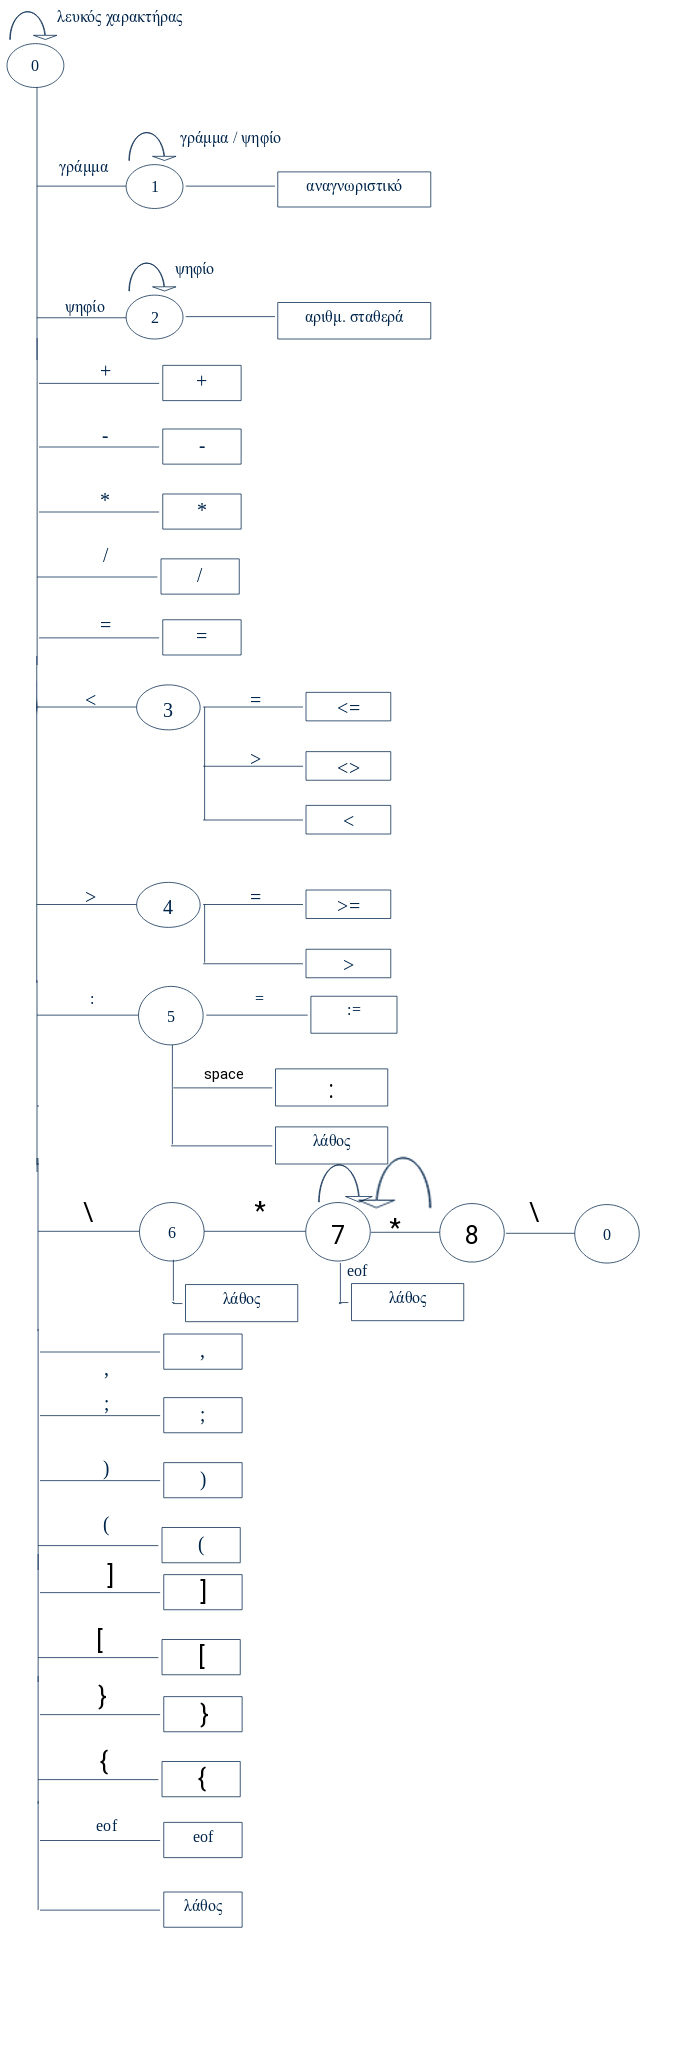
\includegraphics{lexical_diagram}}
    \caption{}
    \label{figure:lexical}
\end{figure}
Η λεκτική ανάλυση πραγματοποιείται στο αρχείο \texttt{lexical.py}. Η βοηθητική
συνάρτηση \texttt{initialize()} ανοίγει το αρχείο που της ζητείται και το αποθηκεύει
σε μία λίστα όπου το κάθε στοιχείο της είναι μία γραμμή του αρχείου. Η συνάρτηση
\texttt{getNextCharacter()} επιστρέφει τον επόμενο χαρακτήρα του αρχείου και
ενημερώνει τις παγκόσμιες μεταβλητές \texttt{currentLine} και
\texttt{currentColumn} για τη θέση του χαρακτήρα μέσα στο αρχείο. Η συνάρτηση
\texttt{ungetCharacter()} αναγκάζει τη συνάρτηση \texttt{getNextCharacter()} να
επιστρέψει ξανά τον ίδιο χαρακτήρα στην επόμενη κλήση της.

Η κύρια συνάρτηση που επιστρέφει το επόμενο λεκτικό στοιχείο είναι η
\texttt{getNextToken()}. Υλοποιεί ένα αυτόματο πεπερασμένων καταστάσεων στο οποίο η
μεταβλητή \texttt{state} καθορίζει την τρέχουσα κατάσταση. Ανάλογα με την τρέχουσα
κατάσταση και το χαρακτήρα που διαβάστηκε, καθορίζεται η επόμενη κατάσταση. Έτσι
αναγνωρίζει αριθμητικές σταθερές, αναγνωριστικά και διάφορα ειδικά σύμβολα της
γλώσσας Ciscal. Επίσης φροντίζει να αναγνωρίζει τα σχόλια που είναι έγκυρα
ορισμένα, αλλιώς εμφανίζει ειδικό μήνυμα λάθους. Επιπλέον, σε κάθε περίπτωση, αν ο
χαρακτήρας δεν είναι επιθυμητός στην τρέχουσα κατάσταση, εμφανίζεται μήνυμα λάθους.
Στο τέλος επιστρέφει ένα αντικείμενο \texttt{Token}. Αυτό έχει τρία πεδία: το
αναγνωριστικό που σχηματίστηκε, τον τύπο του αναγνωριστικού και πληροφορίες
σφάλματος, όπως αυτές ορίζονται παρακάτω.

\newpage
\section{Συντακτική ανάλυση}
Η συντακτική ανάλυση πραγματοποιείται στο αρχείο \texttt{syntax.py}. Για κάθε
κατηγόρημα της γραμματικής της γλώσσας Ciscal υλοποιείται μία αντίστοιχη συνάρτηση.
Αρχικά πρέπει να κληθεί η συνάρτηση \texttt{program()}, που είναι και η αρχική.
Αυτή με τη σειρά της και ανάλογα με το πρόγραμμα προς μετάφραση, φροντίζει να
καλέσει τις απαραίτητες συναρτήσεις. Αυτή η διαδικασία συνεχίζεται μέχρι να
φτάσουμε στα δομικά στοιχεία της γλώσσας (όπως αριθμητικές σταθερές, ή διάφορα
ειδικά σύμβολα). Στη συνέχεια οι συναρτήσεις επιστρέφουν προς τα πάνω, έως όπου να
επιστρέψουμε στην αρχική συνάρτηση \texttt{program()}, όπου αναμένουμε να βρούμε το
τέλος του αρχείου (End-Of-File). Πριν την κλήση κάθε συνάρτησης, είναι υποχρεωτικό να
έχουμε τοποθετήσει στην παγκόσμια μεταβλητή token το επόμενο λεκτικό στοιχείο.
Επίσης, η ίδια δουλειά γίνεται από κάθε συνάρτηση αμέσως πριν την επιστροφή της
(ώστε το επόμενο λεκτικό στοιχείο να είναι έτοιμο για την επόμενη συνάρτηση).
Τέλος, σε όλη τη διάρκεια της συντακτικής ανάλυσης ελέγχουμε εξονυχιστικά για όλα
τα συντακτικά που ενδέχεται να εντοπιστούν. Ενδεικτικά, κάποια από αυτά είναι:
ελλιπής παρενθέσεις, άγκιστρα και αγκύλες, λάθος δεσμευμένες λέξεις της γλώσσας
(π.χ. if, inout, while κ.τ.λ) και χρήση αναγνωριστικών σε σημεία που δε
χρειάζονται.

Πιο αναλυτικά, για κάθε συνάρτηση έχουμε:
\begin{itemize}
    \item \texttt{program():} Είναι η συνάρτηση που καλείται όταν βρίσκουμε
        τη λέξη program κατά τη μεταγλώττιση.
    \item \texttt{block(blockName = None):} Παίρνει σαν προαιρετικό όρισμα
        το όνομα του block και φροντίζει να μεταφράσει κάθε block του
        κώδικα καλώντας τις κατάλληλες συναρτήσεις.
    \item \texttt{declarations():} Διατρέχει τη λίστα δηλώσεων στο
        αντίστοιχο block.
    \item \texttt{varlist():} Διατρέχει μία--μία τις μεταβλητές.
    \item \texttt{subprograms():} Καλεί τη συνάρτηση \texttt{func()} για
        κάθε υποπρόγραμμα.
    \item \texttt{func(isFunction):} Καλεί τη συνάρτηση \texttt{funcbody()}
        για συναρτήσεις και διαδικασίες.
    \item \texttt{funcbody(funcName):} Διατρέχει το κύριο μέρος των
        συναρτήσεων.
    \item \texttt{formalpars():} Διατρέχει τη λίστα των τυπικών παραμέτρων.
    \item \texttt{formalparlist():} Για κάθε παράμετρο που συναντά, καλεί
        τη \texttt{formalparitem()}.
    \item \texttt{formalparitem(allowNothing):} Διαβάζει μία τυπική παράμετρο.
    \item \texttt{sequence():} Καλεί τη \texttt{statement()} για κάθε
        εντολή που συναντάει.
    \item \texttt{brack\_or\_stat():} Διαβάζει μία εντολή που μπορεί να
        περικλείεται σε άγκιστρα ή όχι.
    \item \texttt{statement():} Αποφασίζει για τι είδος εντολής πρόκειται.
    \item \texttt{assignment\_stat(identifier):} Διατρέχει μία εντολή
        ανάθεσης.
    \item \texttt{if\_stat():} Διατρέχει το πρώτο μέρος μίας εντολής if.
    \item \texttt{elsepart():} Διατρέχει το δεύτερο μέρος μίας εντολής if.
    \item \texttt{while\_stat():} Διατρέχει μια εντολή while.
    \item \texttt{select\_stat():} Διατρέχει μια εντολή select.
    \item \texttt{do\_while\_stat():} Διατρέχει μία εντολή do--while.
    \item \texttt{return\_stat():} Διατρέχει μία εντολή return.
    \item \texttt{print\_stat():} Διατρέχει μία εντολή print.
    \item \texttt{call\_stat():} Διατρέχει μία εντολή call.
    \item \texttt{actualpars(functionItem):} Διατρέχει τη λίστα των
        πραγματικών παραμέτρων.
    \item \texttt{actualparlist(functionItem):} Για κάθε παράμετρο που
        συναντά καλεί την \texttt{actual\_par\_item}.
    \item \texttt{actualparitem(allowNothing, functionItem, argumentId):}
        Διαβάζει μια πραγματική παράμετρο.
    \item \texttt{condition():} Διατρέχει μια συνθήκη με or.
    \item \texttt{boolterm():} Διατρέχει μια συνθήκη με and.
    \item \texttt{boolfactor():} Διατρέχει μία συνθήκη με not, ή μια
        συνθήκη που βρίσκεται μέσα σε άγκιστρα, ή μία συνθήκη που
        αποτελείται από δύο εκφράσεις και ένα σχεσιακό τελεστή.
    \item \texttt{expression():} Διατρέχει μία αριθμητική έκφραση που
        αποτελείται από προσθέσεις και αφαιρέσεις.
    \item \texttt{term():} Διατρέχει μία αριθμητική έκφραση που αποτελείται
        από πολλαπλασιασμούς και διαιρέσεις.
    \item \texttt{factor():} Διατρέχει μία αριθμητική σταθερά, ή μία
        έκφραση σε παρενθέσεις, ή μία κλήση συνάρτησης.
    \item \texttt{idtail(identifier):} Διατρέχει πραγματικές παραμέτρους,
        εφόσον υπάρχουν.
    \item \texttt{relational\_oper():} Διατρέχει όλους τους σχεσιακούς
        τελεστές.
    \item \texttt{add\_oper():} Διατρέχει το + και το -.
    \item \texttt{mul\_oper():} Διατρέχει το * και το /.
    \item \texttt{optional\_sign():} Διατρέχει προσημασμένους αριθμούς.
\end{itemize}

Επίσης, χρησιμοποιούμε τις ακόλουθες βοηθητικές συναρτήσεις:
\begin{itemize}
    \item \texttt{getNextToken():} Ζητά το επόμενο λεκτικό στοιχείο από το
        λεκτικό αναλυτή.
    \item \texttt{checkUndeclaredIdentifier():} Ελέγχει για μη δηλωμένα
        αναγνωριστικά.
    \item \texttt{checkAlreadyDeclaredIdentifier():} Ελέγχει για ήδη
        δηλωμένα αναγνωριστικά στο τρέχον βάθος φωλιάσματος.
\end{itemize}

\section{Ενδιάμεσος κώδικας}
Οι βοηθητικές συναρτήσεις που χρειαστήκαμε για τον ενδιάμεσο κώδικα
βρίσκονται στο αρχείο \texttt{intermediate.py}.
\begin{enumerate}
    \item Η \texttt{nextQuad()} μας δίνει τον αριθμό της επόμενης τετράδας
        που θα παραχθεί από το σημείο που βρισκόμαστε.
    \item Η \texttt{newTemp()} μας επιστρέφει την επόμενη διαθέσιμη
        προσωρινή μεταβλητή που θα παραχθεί και δεν χρησιμοποιείται ήδη.
        Αυτό επιτυγχάνεται με χρήση παγκόσμιας μεταβλητής που λειτουργεί ως
        μετρητής.
    \item Η \texttt{emptyList()} δημιουργεί και επιστρέφει μία κενή λίστα
        ετικετών τετράδων. Χρησιμοποιείται όταν δεν γνωρίζουμε ακόμη τον
        προορισμό ενός άλματος.
    \item Η \texttt{makeList(x)} δημιουργεί και επιστρέφει μία λίστα
        ετικετών τετράδων με μοναδικό στοιχείο το x. Χρησιμοποιείται για
        τον ίδιο λόγο με την \texttt{emptyList()}.
    \item Η \texttt{merge(list1, list2)} συνενώνει τις λίστες
        \texttt{list1} και \texttt{list2} σε μία λίστα και την επιστρέφει.
    \item Η \texttt{backPatch(myList, z)} συμπληρώνει το τελευταίο στοιχείο
        κάθε τετράδας στη \texttt{myList} με \texttt{z}.
    \item Επίσης έχουμε συναρτήσεις που γράφουν τον ενδιάμεσο κώδικα που
        παράγεται σε ένα αρχείο καθώς και τον ισοδύναμο κώδικα σε C σε ένα
        διαφορετικό αρχείο. Ο κώδικας C μας βοηθάει στον εύκολο έλεγχο της
        λειτουργίας του κώδικα.
\end{enumerate}

Κατά τη διάρκεια της συντακτικής ανάλυσης παράγεται ο ενδιάμεσος κώδικας
καλώντας τις παραπάνω βοηθητικές συναρτήσεις. Πιο συγκεκριμένα, για τις
παρακάτω περιπτώσεις έχουμε:
\begin{enumerate}
    \item Στην αρχή κάθε μποκ παράγουμε: \\ \texttt{genquad(“
        begin\_block”,name,”\_”,”\_”)} 
    \item Στο τέλος κάθε μπλοκ παράγουμε: \\
        \texttt{genquad(“end\_block”,name,”\_”,”\_”)} \\ Αν πρόκειται για
        το τέλος του προγράμματος, παράγουμε επίσης: \\
        \texttt{genquad(“halt”,”\_”,”\_”,”\_”)}
    \item Στην περίπτωση $ ΕE -> T^1(+T^2\{P_1\})^* \{P_2\}$ παράγουμε \\
        \texttt{$\{P_1\}:  w =
        newTemp()\\ genquad(“+”,T^1.place,T^2.place,w)\\T^1.place=w$ \\
        $\{P_2\}: E.place=T^1.place$} 
	\item Στην περίπτωση $ T -> F^1(xF^2\{P_1\})^* \{P_2\}$ παράγουμε \\
        \texttt{$\{P_1\}:  w =
        newTemp()\\genquad(“x”,F^1.place,F^2.place,w)\\F^1.place=w$ \\
        $\{P_2\}: T.place=F^1.place$}
	\item Στην περίπτωση $ F -> (E) \{P_1\} $ παράγουμε \\
		\texttt{$\{P_1\}: F.place=E.place$}
	\item Στην περίπτωση $ F -> id \{P_1\} $ παράγουμε \\
		\texttt{$\{P_1\}: F.place=id.place$}	
	\item Στην περίπτωση $ B -> Q^1\{P_1\}( or \{P_2\}Q^2 \{P3\})^* $ παράγουμε \\
		\texttt{$\{P_1\}: B.true=Q^1.true \\ B.false=Q^1.false$ \\ 
		$\{P_2\}: backpatch(B.false, nextquad())$ \\
		$\{P_3\}: B.true=merge(B.true, Q^2.true)$ \\ 
		$B.false= Q^2.false$}
	\item Στην περίπτωση $ Q -> R^1\{P_1\}( and \{P_2\}R^2 \{P3\})^* $ παράγουμε \\
		\texttt{$\{P_1\}: Q.true=R^1.true \\ Q.false=R^1.false$ \\ 
		$\{P_2\}: backpatch(Q.true, nextquad())$ \\
		$\{P_3\}: Q.false=merge(Q.false, R^2.false)$ \\ 
		$Q.true= R^2.true$}
	\item Στην περίπτωση $ R -> (B)\{P_1\} $ παράγουμε \\
		\texttt{$\{P_1\}: R.true=B.true \\ R.false=B.false $}
	\item Στην περίπτωση $ R ->E^1relopE^2\{P_1\} $ παράγουμε \\
		\texttt{$\{P_1\}: R.true=makelist(nextquad())$ \\
		$genquad(relop, E^1.place, E^2.place, “\_”) $ \\ 
		$R.false=makelist(nextquad()) $ \\
		$genquad(“jump” , “\_” , “\_” , “\_”)$}
	\item Στην περίπτωση που έχουμε κλήση διαδικασίας, για παράδειγμα: $call$ $assign\_v(in a, inoutb)$ 
		παράγουμε \\ \texttt{$par, a, CV, "\_" \\ par, b, REF, "\_" \\ call, assign\_v, "\_", "\_" $}
	\item Στην περίπτωση που έχουμε κλήση συνάρτησης, για παράδειγμα: $error = assign\_v(in a, inoutb)$ 	
		παράγουμε \\ \texttt{$par, a, CV, "\_" \\ par, b, REF, "\_" \\ w = newTemp() \\ par, w, RET, "\_" 			\\ call, assign\_v, "\_", "\_" $}
	\item Στην περίπτωση $ S -> return (E) \{P_1\} $ παράγουμε \\ 
		\texttt{$ \{P_1\}:genquad(“retv”,E.place,”\_”,”\_”) $}
	\item Στην περίπτωση $ S-> id := E \{P_1\} $ παράγουμε \\ 
		\texttt{$ \{P_1\}:genquad(“:=“,E.place,”\_”,id) $}	
	\item Στην περίπτωση  $ S -> while \{P_1\}B do \{P_2\}S^1\{P_3\} $ παράγουμε \\
		\texttt{$ \{P_1\}: Bquad:=nextquad() \\ \{P_2\}: backpatch(B.true,nextquad()) \\ \{P_3\}: 
		genquad(“jump”,”\_”,”\_”,Bquad) \\ backpatch(B.false,nextquad()) $}
	\item Στην περίπτωση  $ S -> repeat \{P_1\}S^1$ $until (cond) \{P_2\} $ παράγουμε \\	
		\texttt{$ \{P_1\}: sQuad:=nextquad() \\ \{P_2\}: backpatch(cond.False,sQuad) \\ 			 
		backpatch(cond.True,nextquad()) $}
	\item Στην περίπτωση  $ S -> if B then \{P_1\} S^1 \{P_2\}TAIL \{P_3\}$ ,'οπου: $TAIL -> else S^2$ $|$ 
		$ TAIL -> e $ παράγουμε \\ 
		\texttt{$ \{P_1\}: backpatch(B.true,nextquad()) \\ \{P_2\}: ifList=makelist(nextquad()) \\
		genquad(“jump”,”\_”,”\_”,”\_”) \\ backpatch(B.false,nextquad()) \\ \{P_3\}: 
		backpatch(ifList,nextquad()) $}
	\item Στην περίπτωση  $ S -> input (id) \{P_1\} $ παράγουμε \\ 
		\texttt{$ \{P_1\}: genquad(“inp”,id.place,”\_”,”\_”) $}
	\item Στην περίπτωση  $ S -> print(E) \{P_1\} $ παράγουμε \\ 
		\texttt{$ \{P_1\}: genquad(“out”,E.place,”\_”,”\_”) $}
			
\end{enumerate}

\section{Πίνακας Συμβόλων}
Για τον πίνακα συμβόλων έχουμε υλοποιήσει τρεις κλάσεις καθώς και τις
απαραίτητες βοηθητικές συναρτήσεις μέσα στο αρχείο \texttt{symbolTable.py}. 

Στην κλάση EntityItem δημιουργόυμε το κατάλληλο αντικείμενο ανάλογα με τον
τύπο της οντότητας. 
\begin{enumerate}
    \item Αν είναι \emph{παράμετρος} κρατάμε τις πληροφορίες
        \texttt{itemType, itemName, isIn} και \texttt{offset}.
    \item Αν είναι \emph{συνάρτηση}, κρατάμε τις πληροφορίες
        \texttt{itemType, itemName, isFunction, startQuad, argumentList}
        και \texttt{frameLength}.
    \item Αν είναι \emph{μεταβλητή}, κρατάμε τις πληροφορίες
        \texttt{itemType, itemName} και \texttt{offset}.
\end{enumerate}

Στην κλάση \texttt{ScopeItem} κρατάμε μία λίστα από \texttt{Entities} και
έχουμε 2 βοηθητικές μεθόδους ώστε να προσθέτουμε \texttt{Entity} ή να
προσθέτουμε \texttt{Argument}.

Στην κλάση \texttt{ArgumentItem}  κρατάμε αν η παράμετρος περνιέται με τιμή
ή με αναφορά χρησιμοποιώντας μία boolean μεταβλητή.

Στο Σχήμα \ref{figure:symbol} φαίνεται διαγραμματικά ένα παράδειγμα του
πίνακα συμβόλων εν ώρα εκτέλεσης. Οι κόκκινοι κύκλοι αναπαριστούν
αντικείμενα τύπου \texttt{ScopeItem}, τα κίτρινα ορθογώνια αναπαριστούν
αντικείμενα τύπου \texttt{EntityItem}, ενώ τα γαλάζια τρίγωνα αναπαριστούν
αντικείμενα τύπου \texttt{Argu\-mentItem}. 
\begin{figure}[!htpb]
    \resizebox{5in}{!}{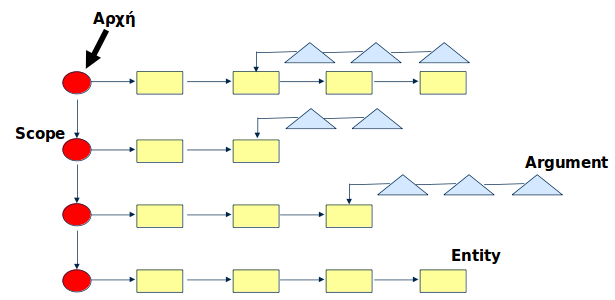
\includegraphics{symbol_table}}
    \caption{Ο πίνακας συμβόλων εν ώρα εκτέλεσης}
    \label{figure:symbol}
\end{figure}

Τέλος, παρέχουμε βοηθητικές συναρτήσεις που προσθέτουν, αφαιρούν και
τροποποιούν αντικείμενα των παραπάνω κλάσεων και αναζητούν πληροφορίες μέσα
στον πίνακα συμβόλων για δοθέντα elements.

\section{Τελικός κώδικας}
Ο τελικός κώδικας και οι βοηθητικές συναρτήσεις που χρησιμοποιεί
υλοποιούνται στο αρχείο \texttt{final.py}.

Η συνάρτηση \texttt{gnvlcode()} μεταφέρει στον καταχωρητή \texttt{\$t0} τη
διεύθυνση μιας μη τοπικής μεταβλητής την οποία παίρνει ως παράμετρο. Για να
το επιτύχει αυτό αρχικά βρίσκει τη μεταβλητή στον πίνακα συμβόλων. Στη
συνέχεια, παράγουμε εντολές τελικού κώδικα ώστε να βρεθούμε στη
στοίβα\footnote{μια εικόνα της στοίβας για μία συνάρτηση σε χρόνο εκτέλεσης
φαίνεται στο Σχήμα \ref{figure:stack}} του γονέα και μετά, για όσες φορές
χρειαστεί μέχρι να φτάσουμε στη στοίβα του προγόνου που περιέχει τη
ζητούμενη μεταβλητή. Τέλος, με χρήση του offset της μεταβλητής βρίσκουμε
ακριβώς το σημείο που βρίσκεται η μεταβλητή.
\begin{figure}[!htpb]
    \resizebox{3in}{!}{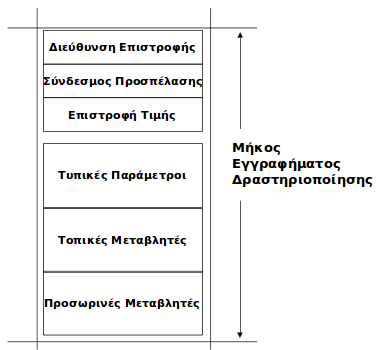
\includegraphics{stack}}
    \caption{Η στοίβα μιας συνάρτησης σε χρόνο εκτέλεσης}
    \label{figure:stack}
\end{figure}

Η συνάρτηση \texttt{loadvr(v, r)} μεταφέρει τη διεύθυνση μιας μεταβλητής v στον
καταχωρητή r. Για να το καταφέρουμε αυτό, διακρίνουμε τις εξής περιπτώσεις:
\begin{enumerate}
\item Αν είναι σταθερά, απλά φορτώνουμε την τιμή της στον καταχωρητή.
\item Αν είναι καθολική μεταβλητή, φορτώνουμε την τιμή της χρησιμοποιώντας το
offset της, αλλά και τον καταχωρητή \texttt{\$s0}, στον οποίο έχουμε
αποθηκεύσει ένα δείκτη στη στοίβα της main.
\item Αν είναι τοπική μεταβλητή, ή τυπική παράμετρος που περνάει με τιμή και βάθος 
φωλιάσματος ίσο με το τρέχον, ή προσωρινή μεταβλητή, τότε τη φορτώνουμε
χρησιμοποιώντας το offset της από την τρέχουσα στοίβα.
\item Αν είναι τυπική παράμετρος που περνάει με αναφορά και βάθος φωλιάσματος
ίσο με το τρέχον, τότε αρχικά φορτώνουμε τη διεύθυνσή της χρησιμοποιώντας
το offset της από την τρέχουσα στοίβα και στη συνέχεια φορτώνουμε την τιμή
στην οποία δείχνει αυτή η διεύθυνση.
\item Αν είναι τοπική μεταβλητή, ή τυπική παράμετρος που περνάει με τιμή και
βάθος φωλιάσματος μικρότερο από το τρέχον, τότε αρχικά φορτώνουμε τη
διεύθυνσή της χρησιμοποιώντας τη βοηθητική συνάρτηση \texttt{gnlvcode()}
και στη συνέχεια φορτώνουμε την τιμή στην οποία δείχνει αυτή η διεύθυνση.
\item Αν είναι τυπική παράμετρος που περνάει με αναφορά και βάθος φωλιάσματος
μικρότερο από το τρέχον, τότε αρχικά φορτώνουμε τη
διεύθυνσή της χρησιμοποιώντας τη βοηθητική συνάρτηση \texttt{gnlvcode()},
και στη συνέχεια φορτώνουμε την τιμή στην οποία δείχνει αυτή η διεύθυνση
στον καταχωρητή r.
\end{enumerate}

Η συνάρτηση \texttt{storerv(r, v)} μεταφέρει τη διεύθυνση μιας μεταβλητής v στον
καταχωρητή r. Για να το καταφέρουμε αυτό, διακρίνουμε τις εξής περιπτώσεις:
\begin{enumerate}
\item Αν είναι σταθερά, απλά αποθηκεύουμε την τιμή του στη μεταβλητή.
\item Αν είναι τοπική μεταβλητή, ή τυπική παράμετρος που περνάει με τιμή και βάθος 
φωλιάσματος ίσο με το τρέχον, ή προσωρινή μεταβλητή, τότε αποθηκεύουμε την
τιμή του χρησιμοποιώντας το offset του από την τρέχουσα στοίβα.
\item Αν είναι τυπική παράμετρος που περνάει με αναφορά και βάθος φωλιάσματος
ίσο με το τρέχον, τότε αρχικά φορτώνουμε τη διεύθυνσή της χρησιμοποιώντας
το offset της από την τρέχουσα στοίβα και στη συνέχεια αποθηκεύουμε την τιμή
του στη διεύθυνση που δείχνει.
\item Αν είναι τοπική μεταβλητή, ή τυπική παράμετρος που περνάει με τιμή και
βάθος φωλιάσματος μικρότερο από το τρέχον, τότε αρχικά φορτώνουμε τη
διεύθυνσή της χρησιμοποιώντας τη βοηθητική συνάρτηση \texttt{gnlvcode()}
και στη συνέχεια αποθηκεύουμε την τιμή του στη διεύθυνση που δείχνει.
\item Αν είναι τυπική παράμετρος που περνάει με αναφορά και βάθος φωλιάσματος
μικρότερο από το τρέχον, τότε αρχικά φορτώνουμε τη
διεύθυνσή της χρησιμοποιώντας τη βοηθητική συνάρτηση \texttt{gnlvcode()},
και στη συνέχεια φορτώνουμε τη διεύθυνση που είναι αποθηκευμένη η τιμή που
χρειαζόμαστε και στη συνέχεια αποθηκεύουμε τα περιεχόμενα του καταχωρητή r
σε αυτή την τιμή.
\end{enumerate}

Η συνάρτηση \texttt{generateFinalCode()} παράγει τελικό κώδικα για τις
διάφορες εντολές ενδιάμεσου κώδικα που μπορεί να συναντήσει. Διακρίνουμε
τις παρακάτω περιπτώσεις:
\begin{enumerate}
    \item \texttt{jump, “\_”, “\_”, label} \\ Παράγουμε την εντολή \\
        \texttt{j label} 
    \item \texttt{relop (?), x,y,z} \\ Παράγουμε τις εντολές \\
        \texttt{loadvr(x,1) \\ loadvr(y,2) \\ branch(?),\$t1,\$t2,z}, όπου
        branch(?) είναι μία από τις εντολές \texttt{beq, bne, bgt, blt,
        bge, ble}
    \item \texttt{:=, x, “\_”, z} \\ Παράγουμε τις εντολές \\
        \texttt{loadvr(x,1) \\ storerv(1,z)} 
    \item \texttt{op x,y,z} \\ Παράγουμε τις εντολές \\ \texttt{loadvr(x,1)
        \\ loadvr(y,2) \\ op \$t1,\$t1,\$t2 \\ storerv(1,z)}, όπου op είναι
        μία από τις εντολές add,sub,mul,div
    \item \texttt{out “\_”, “\_”, x} \\ Παράγουμε τις εντολές \\ \texttt{li
        \$v0,1 \\ li \$a0, x \\ syscall} 
    \item \texttt{in “\_”, “\_”, x} \\ Παράγουμε τις εντολές \\ \texttt{li
        \$v0,5 \\ syscall} 
    \item \texttt{retv “\_”, “\_”, x} \\ Παράγουμε τις εντολές\\
        \texttt{loadvr(x,1) \\ lw \$t0, -8(\$sp) \\ sw \$t1,(\$t0)} 
    \item Πριν από την πρώτη παράμετρο, τοποθετούμε τον \texttt{\$fp} να
        δείχνει στην στοίβα της συνάρτησης που θα δημιουργηθεί \texttt{add
        \$fp,\$sp,framelength}. Στη συνέχεια διακρίνουμε υποπεριπτώσεις:
    \begin{enumerate}
        \item \texttt{par,x,CV , \_} \\ Παράγουμε τις εντολές \\
            \texttt{loadvr(x,0) \\ sw \$t0, -(12+4i)(\$fp)}, όπου i ο αύξων
            αριθμός της παραμέτρου
        \item \texttt{par,x,REF , \_} \\ Διακρίνουμε τις υποπεριπτώσεις:
            \begin{itemize}
                \item Αν η καλούσα συνάρτηση και η μεταβλητή x έχουν το
                    ίδιο βάθος φωλιάσματος, η παράμετρος x είναι στην
                    καλούσα συνάρτηση τοπική μεταβλητή ή παράμετρος που
                    έχει περαστεί με τιμή, παράγουμε τις εντολές \\
                    \texttt{add \$t0,\$sp, -offset \\ sw \$t0,
                    -(12+4i)(\$fp)} 
                \item Αν η καλούσα συνάρτηση και η μεταβλητή x έχουν το
                    ίδιο βάθος φωλιάσματος, η παράμετρος x είναι στην
                    καλούσα συνάρτηση παράμετρος που έχει περαστεί με
                    αναφορά παράγουμε τις εντολές \\ \texttt{lw \$t0,
                    -offset(\$sp) \\ sw \$t0, -(12+4i)(\$fp)}
                \item Αν η καλούσα συνάρτηση και η μεταβλητή x έχουν
                    διαφορετικό βάθος φωλιάσματος, η παράμετρος x είναι
                    στην καλούσα συνάρτηση τοπική μεταβλητή ή παράμετρος
                    που έχει περαστεί με τιμή, παράγουμε τις εντολές \\ 
                    \texttt{gnlvcode(x) \\ sw \$t0, -(12+4i)(\$fp)}
                \item Αν η καλούσα συνάρτηση και η μεταβλητή x έχουν
                    διαφορετικό βάθος φωλιάσματος, η παράμετρος x είναι
                    στην καλούσα συνάρτηση παράμετρος που έχει περαστεί με
                    αναφορά, παράγουμε τις εντολές \\ \texttt{gnlvcode(x)
                    \\ lw \$t0,(\$t0) \\ sw \$t0, -(12+4i)(\$fp)}
            \end{itemize}
        \item \texttt{par,x,RET , \_} \\ Παράγουμε τις εντολές \\
            \texttt{add \$t0,\$sp, -offset \\ sw \$t0, -8(\$fp)}
    \end{enumerate}
    \item \texttt{call, \_, \_, f} \\ Διακρίνουμε τις υποπεριπτώσεις:
    \begin{itemize}
        \item Αν καλούσα και κληθείσα έχουν το ίδιο βάθος φωλιάσματος, τότε
            έχουν τον ίδιο γονέα και παράγουμε τις εντολές \\ \texttt{lw
            \$t0, -4(\$sp) \\ sw \$t0, -4(\$fp)}
        \item Αν καλούσα και κληθείσα έχουν διαφορετικό βάθος φωλιάσματος,
            τότε η καλούσα είναι ο γονέας της κληθείσας και παράγουμε τις
            εντολές \\ \texttt{sw \$sp, -4(\$fp)} 
    \end{itemize}

    Στη συνέχεια μεταφέρουμε τον δείκτη στοίβας στην κληθείσα με την εντολή
    \\ \texttt{add \$sp,\$sp,framelength} \\ Έπειτα καλούμε τη συνάρτηση f με
    την εντολή \texttt{jal f} και όταν επιστρέψουμε παίρνουμε πίσω τον
    δείκτη στοίβας στην καλούσα συνάρτηση με την εντολή \\ \texttt{add
    \$sp,\$sp ,-framelength}

    Μέσα στην κληθείσα στην αρχή κάθε συνάρτησης αποθηκεύουμε στην πρώτη
    θέση του εγγραφήματος δραστηριοποίησης την διεύθυνση επιστροφής της την
    οποία έχει τοποθετήσει στον \$ra η jal με την εντολή \\ \texttt{sw \$ra
    ,(\$sp)} \\ Στo τέλος κάθε συνάρτησης κάνουμε το αντίστροφο, παίρνουμε
    από την πρώτη θέση του εγγραφήματος δραστηριοποίησης την διεύθυνση
    επιστροφής της συνάρτησης και την βάζουμε πάλι στον \$ra. Μέσω του \$ra
    επιστρέφουμε στην καλούσα με τις εντολές \\ \texttt{lw \$ra ,(\$sp) \\ jr \$ra} 

    \item Το κυρίως πρόγραμμα δεν είναι το πρώτο πράγμα που μεταφράζεται,
        οπότε στην αρχή του προγράμματος χρειάζεται ένα άλμα που να οδηγεί
        στην πρώτη ετικέτα του κυρίως προγράμματος με την εντολή \\ \texttt{j
        Lmain} \\ Στη συνέχεια πρέπει να κατεβάσουμε τον \$sp κατά
        framelength της main με την εντολή \\ \texttt{add
        \$sp,\$sp,framelength} \\ και να σημειώσουμε στον \$s0 το εγγράφημα
        δραστηριοποίησης της main ώστε να έχουμε εύκολη πρόσβαση στις
        global μεταβλητές με την εντολή \\ \texttt{move \$s0,\$sp} 
\end{enumerate}

\section{Παρουσίαση μηνυμάτων σφάλματος}
Στο αρχείο \texttt{error.py} ορίζεται η δομή \texttt{ErrorData} καθώς και η
συνάρτηση \texttt{error()} που χρησιμοποιούνται στα υπόλοιπα μέρη του
μεταφραστή για την παρουσίαση σφαλμάτων στο χρήστη. Η δομή
\texttt{ErrorData} αποτελείται από τρία πεδία: το αρχείο πηγαίου κώδικα
Ciscal, τη γραμμή και τη στήλη μέσα σε αυτό το αρχείο όπου συνέβη το
σφάλμα. Η συνάρτηση \texttt{error()} δέχεται ως παραμέτρους την περιγραφή
του σφάλματος και ένα αντικείμενο \texttt{ErrorData} και τυπώνει το αρχείο,
τη γραμμή και τη στήλη που έγινε το σφάλμα, καθώς και την περιγραφή του
σφάλματος. Επίσης ενημερώνει το χρήστη ότι η διαδικασία της μετάφρασης δεν
ήταν επιτυχής και τον παροτρύνει να διορθώσει το πρόβλημα και να
προσπαθήσει ξανά. Η μετάφραση τερματίζεται στο πρώτο σφάλμα.

\end{document}
